%\documentclass[10pt]{beamer}
\documentclass[10pt,aspectratio=169,usenames,dvipsnames]{beamer}

\usetheme[progressbar=frametitle]{metropolis}
\usepackage{appendixnumberbeamer}

\usepackage{booktabs}
\usepackage[scale=2]{ccicons}

\usepackage{pgfplots}
\usepgfplotslibrary{dateplot}

\usepackage{xspace}
\newcommand{\themename}{\textbf{\textsc{metropolis}}\xspace}

\usepackage{graphicx}

\setbeamertemplate{enumerate items}[circle]

\usepackage{pict2e}

\usepackage{media9}

\usepackage{amsmath}

\usepackage{mathtools}
\DeclarePairedDelimiter\abs{\lvert}{\rvert}%
\DeclarePairedDelimiter\norm{\lVert}{\rVert}%
\makeatletter
\let\oldabs\abs
\def\abs{\@ifstar{\oldabs}{\oldabs*}}

\usepackage[makeroom]{cancel}

\usepackage{xcolor}
\usepackage{soul}
\newcommand{\mathcolorbox}[2]{\colorbox{#1}{$\displaystyle #2$}}

\title{Partially ionised shocks with collisional and radiative ionisation and recombination}
%ABSTRACT: 
\date{}
\author{\textbf{Ben Snow}}
\institute{University of Exeter \\ RAS discussion meeting, 13th January 2023.}

\begin{document}

\maketitle

\begin{frame}{Shocks in magnetic reconnection}
\begin{columns}
\begin{column}{0.5\textwidth}
\begin{itemize}
    \item Magnetic reconnection is important for flares.
    \item Shocks are common features of magnetic reconnection (Petschek1964, Shibyama+2015).
    \item Chromosphere is partially ionised - ions and neutrals follow different equations.
    \item Two-fluid shocks not well understood.
\end{itemize}
\end{column}
\begin{column}{0.5\textwidth}
%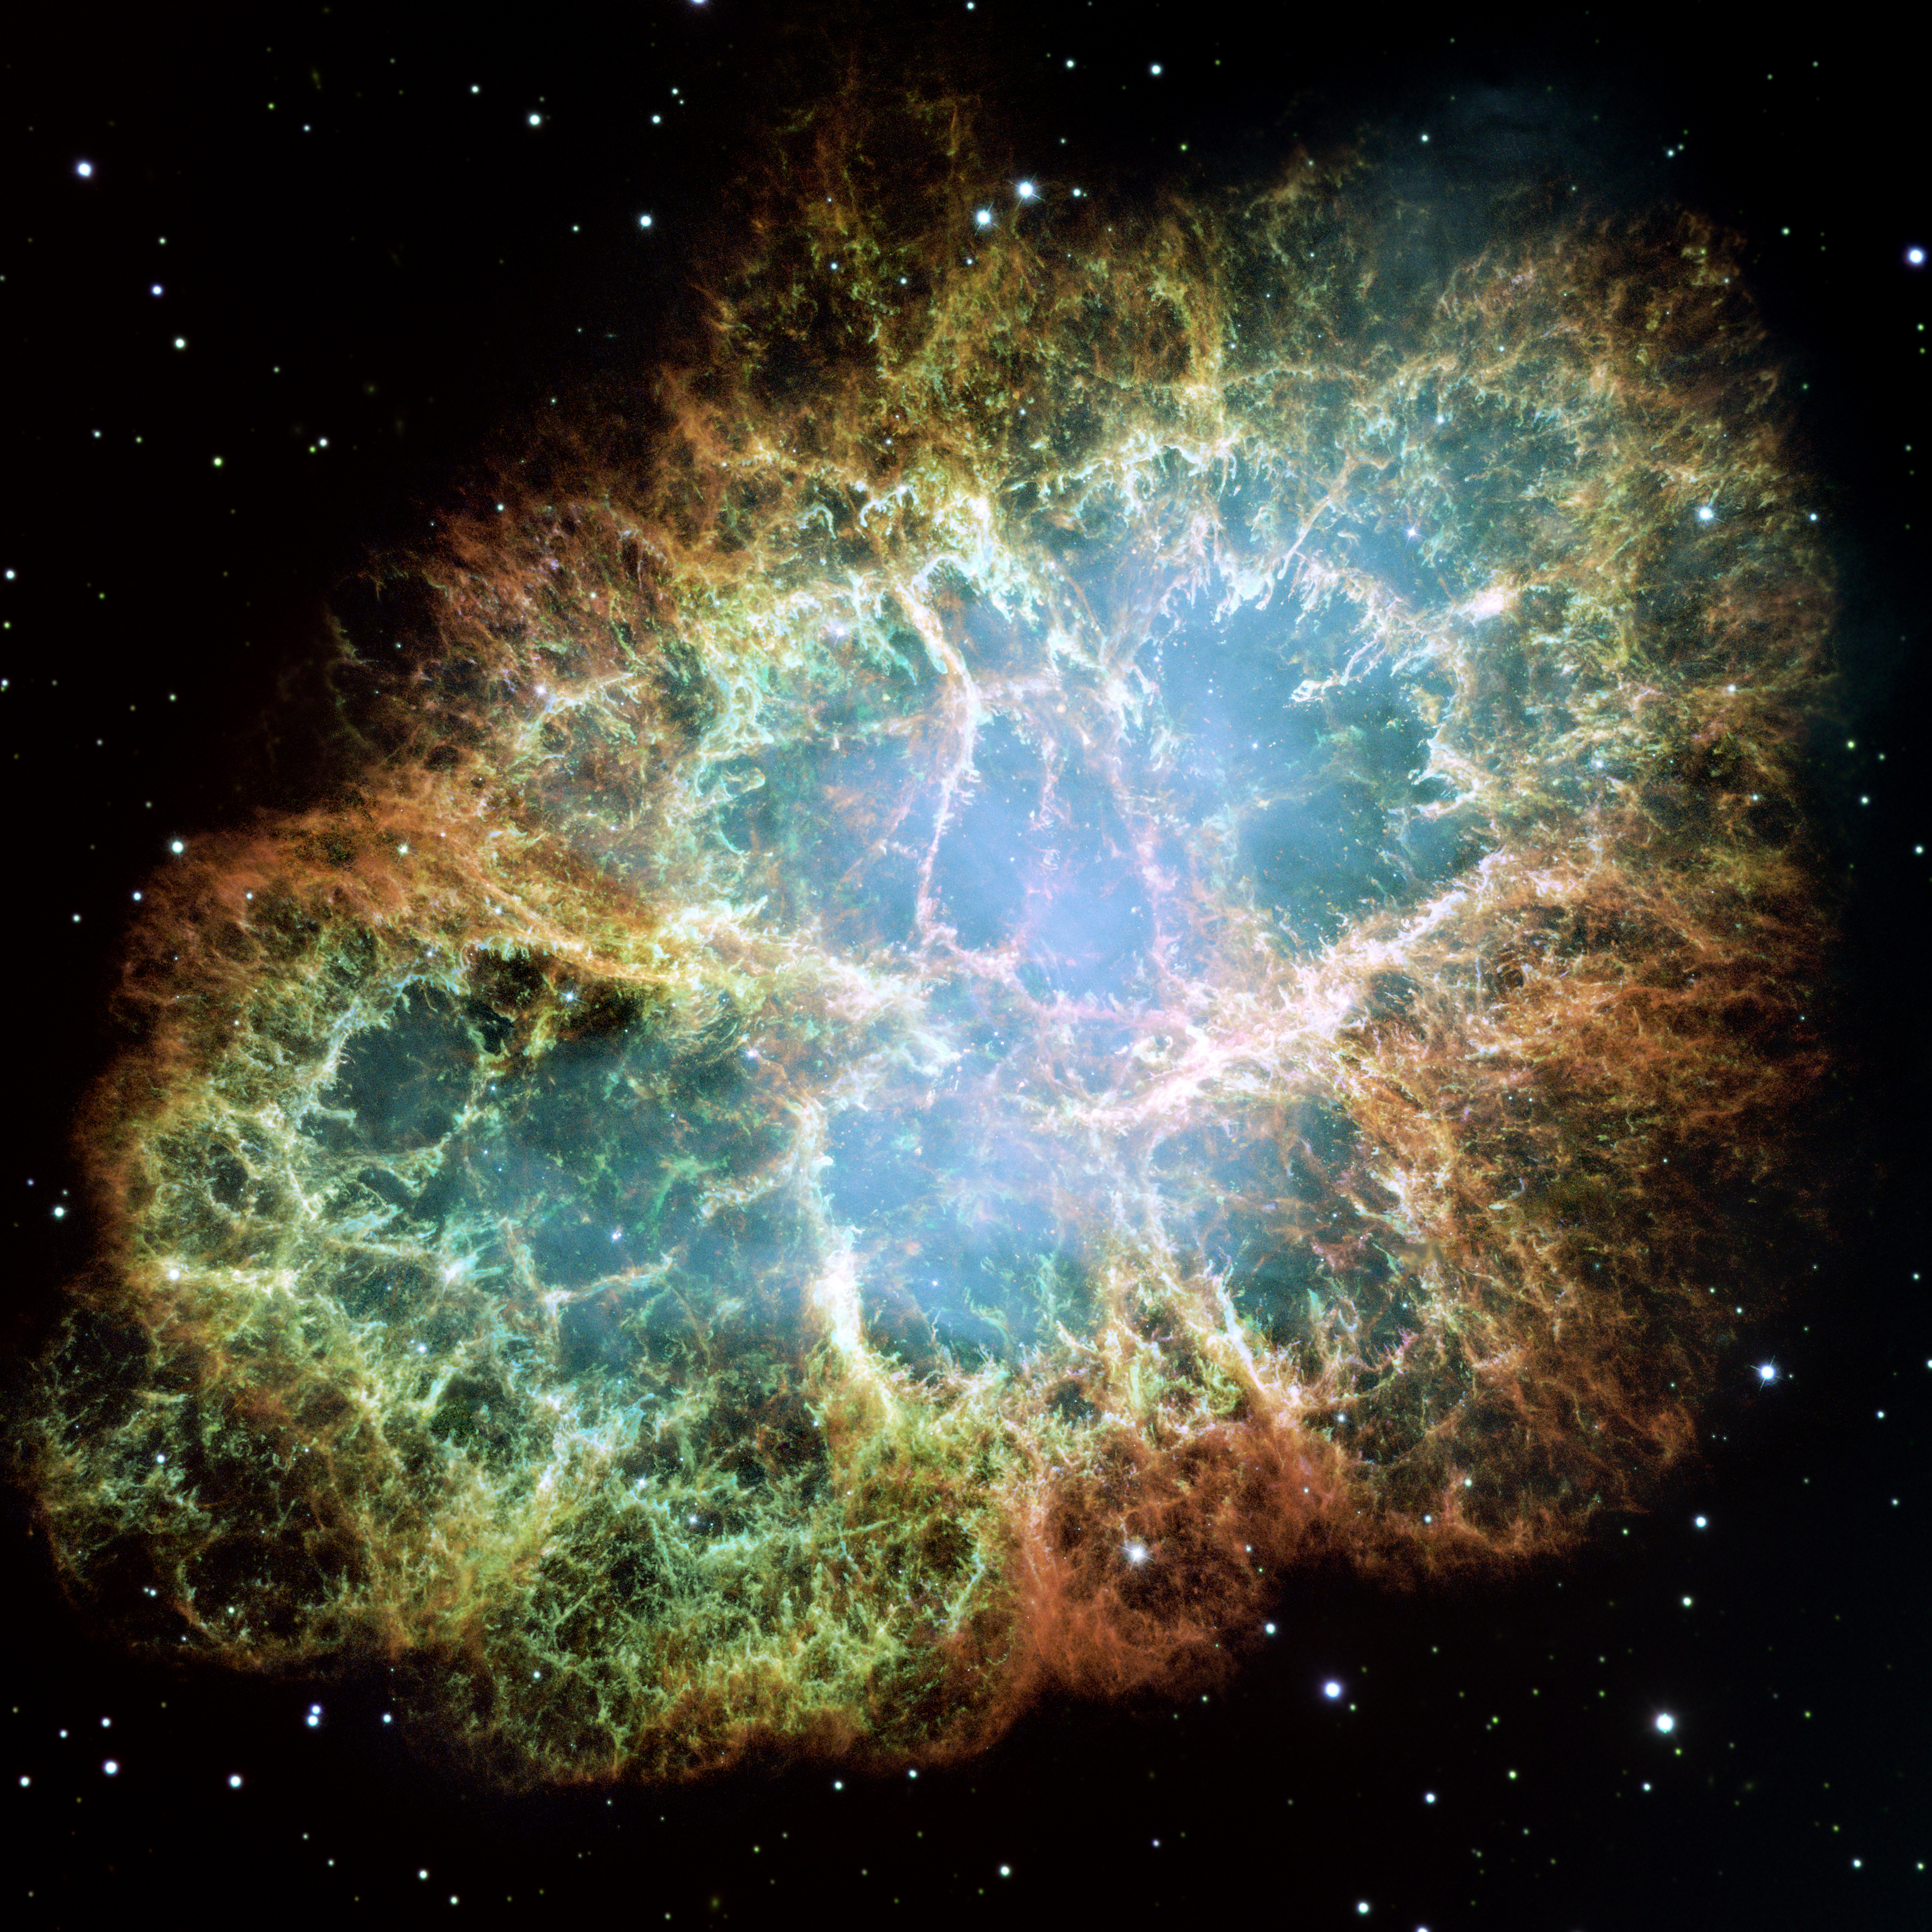
\includegraphics[width=0.32\linewidth]{Figures/Crab_Nebula.jpeg}
\includegraphics[width=0.95\linewidth]{2023RAS/Figures/petschek.png} \\
\includegraphics[width=0.95\linewidth]{2023RAS/Figures/shibyama.png}
%\includegraphics[width=0.32\linewidth]{Figures/cmesketch.jpg}
\end{column}
\end{columns}
\end{frame}

\begin{frame}{Two-fluid shocks - overview}
\begin{columns}
\begin{column}{0.4\textwidth}
\begin{itemize}
    % \item Solar chromosphere is partially ionised.
    % \item Understanding two-fluid shocks is fundamental to understanding energy transfer and heating in the solar chromosphere and corona.
    \item Two-fluid shocks have a finite width as opposed to the discontinuous single-fluid MHD case.
    \item Same overall shock jump but substructure exists.
    \item Ionisation/recombination rates increased in shocks - needs to be considered.
    \item Multiple excited neutral hydrogen states, non-equilibrium ionisation, ionisation/excitation cooling, recombination/de-excitation heating..... 
%    \item Substructure possible.
\end{itemize}
%\includegraphics[width=1.0\textwidth,clip=true,trim=1.0cm 1.0cm 1.0cm 1.0cm]{obs_shockloc_contour.png}
\end{column}
\begin{column}{0.6\textwidth}
%\includegraphics[width=0.95\linewidth,clip=true,trim=0.9cm 7.8cm 1.5cm 7.8cm]{poster_comp.pdf} \\
\includegraphics[width=0.95\linewidth]{Figures/shocksub_col.png} \\
Conservative equations (e.g., two-fluid with thermal collisions) leads to MHD shock jumps, Snow \& Hillier 2019.
\end{column}
\end{columns}
\end{frame}

\begin{frame}{Aims}
\begin{itemize}
    \item Multiple-level, non-equilibrium hydrogen model for ionisation/recombination using collsional/radiative rates in two-fluid framework.
    \item Study how the temperature changes across a partially ionised shock.
    \item See how the temperature jump varies with atmospheric height.
\end{itemize}
\end{frame}

%%%%%%%%%%%%%%%%%%%%%%%%%%%%%%%%%%%%%%%%%%%%%%%%%%%%%%%%%%%%%%%%%%%%%%%%%%%%%%%%%%

\begin{frame}{Ionisation, recombination and ionisation potential in two-fluid shocks}
\footnotesize
\begin{gather}
\frac{\partial \rho _{\text{n}}}{\partial t} + \nabla \cdot (\rho _{\text{n}} \textbf{v}_{\text{n}})= \Gamma _{rec} \rho _{\rm p} - \Gamma _{ion} \rho _{\rm n}, \label{eqn:neutral1}\tag{5} \\
\frac{\partial}{\partial t}(\rho _{\text{n}} \textbf{v}_{\text{n}}) + \nabla \cdot (\rho _{\text{n}} \textbf{v}_{\text{n}} \textbf{v}_{\text{n}} + P_{\text{n}} \textbf{I}) = -\alpha _c \rho_{\text{n}} \rho_{\text{p}} (\textbf{v}_{\text{n}}-\textbf{v}_{\text{p}}) + \Gamma _{rec} \rho _{\rm p} \textbf{v}_{\rm p} - \Gamma _{ion} \rho_{\rm n} \textbf{v}_{\rm n}, \tag{6}\\
\frac{\partial e_{\text{n}}}{\partial t} + \nabla \cdot \left[\textbf{v}_{\text{n}} (e_{\text{n}} +P_{\text{n}}) \right] = -\alpha _c \rho _{\text{n}} \rho _{\text{p}} \left[ \frac{1}{2} (\textbf{v}_{\text{n}} ^2 - \textbf{v}_{\text{p}} ^2)+ \frac{3}{2} \left(\frac{P_{\rm n}}{\rho_{\rm n}}-\frac{1}{2}\frac{P_{\rm p}}{\rho_{\rm p}}\right) \right] \nonumber \\ \hspace{0.5cm}+ \frac{1}{2} \left( \Gamma _{rec} \rho _{\rm p} \textbf{v}_{\rm p} ^2 - \Gamma _{ion} \rho _{\rm n} \textbf{v}_{\rm n} ^2 \right) +\frac{1}{ (\gamma-1)} \left( \frac{1}{2} \Gamma _{rec} P_{\rm p} -\Gamma _{ion} P_{\rm n} \right), \tag{7}\\
%e_{\text{n}} = \frac{P_{\text{n}}}{\gamma -1} + \frac{1}{2} \rho _{\text{n}} v_{\text{n}} ^2, \label{eqn:neutral2} \\
\frac{\partial \rho _{\text{p}}}{\partial t} + \nabla \cdot (\rho_{\text{p}} \textbf{v}_{\text{p}}) = - \Gamma _{rec} \rho _{\rm p} + \Gamma _{ion} \rho _{\rm n} \label{eqn:plasma1}\tag{8}\\
\frac{\partial}{\partial t} (\rho_{\text{p}} \textbf{v}_{\text{p}})+ \nabla \cdot \left( \rho_{\text{p}} \textbf{v}_{\text{p}} \textbf{v}_{\text{p}} + P_{\text{p}} \textbf{I} - \textbf{B B} + \frac{\textbf{B}^2}{2} \textbf{I} \right) = \alpha _c \rho_{\text{n}} \rho_{\text{p}}(\textbf{v}_{\text{n}} - \textbf{v}_{\text{p}}) - \Gamma _{rec} \rho _{\rm p} \textbf{v}_{\rm p} + \Gamma _{ion} \rho_{\rm n} \textbf{v}_{\rm n},\tag{9}\\
\frac{\partial}{\partial t} \left( e_{\text{p}} + \frac{\textbf{B}^2}{2} \right) + \nabla \cdot \left[ \textbf{v}_{\text{p}} ( e_{\text{p}} + P_{\text{p}}) -  (\textbf{v}_{\rm p} \times \textbf{B}) \times \textbf{B} \right]  =  \alpha _c \rho _{\text{n}} \rho _{\text{p}} \left[ \frac{1}{2} (\textbf{v}_{\text{n}} ^2 - \textbf{v}_{\text{p}} ^2)+ \frac{3}{2} \left(\frac{P_{\rm n}}{\rho_{\rm n}}-\frac{1}{2}\frac{P_{\rm p}}{\rho_{\rm p}}\right) \right] \nonumber \\ \hspace{0.5cm}- \frac{1}{2} \left( \Gamma _{rec} \rho _{\rm p} \textbf{v}_{\rm p} ^2 - \Gamma _{ion} \rho _{\rm n} \textbf{v}_{\rm n} ^2 \right) {- \phi_I + \phi_{heat}} -\frac{1}{ (\gamma-1)} \left( \frac{1}{2} \Gamma _{rec} P_{\rm p} -\Gamma _{ion} P_{\rm n} \right), \label{eqn:ep}\tag{10} \\
\frac{\partial \textbf{B}}{\partial t} - \nabla \times (\textbf{v}_{\text{p}} \times \textbf{B}) = 0.\tag{11}
%e_{\text{p}} = \frac{P_{\text{p}}}{\gamma -1} + \frac{1}{2} \rho _{\text{p}} v_{\text{p}} ^2, \\
%\nabla \cdot \textbf{B} = 0,\label{eqn:plasma2}
\end{gather}
\end{frame}

\begin{frame}{Ionisation, recombination and ionisation potential in two-fluid shocks}
\vspace{-0.5cm}
\footnotesize
\begin{gather}
\mathcolorbox{VioletRed}{\frac{\partial \rho _{\text{n}}}{\partial t} + \nabla \cdot (\rho _{\text{n}} \textbf{v}_{\text{n}})}= \Gamma _{rec} \rho _{\rm p} - \Gamma _{ion} \rho _{\rm n}, \label{eqn:neutral1}\tag{5} \\
\mathcolorbox{VioletRed}{\frac{\partial}{\partial t}(\rho _{\text{n}} \textbf{v}_{\text{n}}) + \nabla \cdot (\rho _{\text{n}} \textbf{v}_{\text{n}} \textbf{v}_{\text{n}} + P_{\text{n}} \textbf{I})} = -\alpha _c \rho_{\text{n}} \rho_{\text{p}} (\textbf{v}_{\text{n}}-\textbf{v}_{\text{p}}) + \Gamma _{rec} \rho _{\rm p} \textbf{v}_{\rm p} - \Gamma _{ion} \rho_{\rm n} \textbf{v}_{\rm n}, \tag{6}\\
\mathcolorbox{VioletRed}{\frac{\partial e_{\text{n}}}{\partial t} + \nabla \cdot \left[\textbf{v}_{\text{n}} (e_{\text{n}} +P_{\text{n}}) \right]} = -\alpha _c \rho _{\text{n}} \rho _{\text{p}} \left[ \frac{1}{2} (\textbf{v}_{\text{n}} ^2 - \textbf{v}_{\text{p}} ^2)+ \frac{3}{2} \left(\frac{P_{\rm n}}{\rho_{\rm n}}-\frac{1}{2}\frac{P_{\rm p}}{\rho_{\rm p}}\right) \right] \nonumber \\ \hspace{0.5cm}+ \frac{1}{2} \left( \Gamma _{rec} \rho _{\rm p} \textbf{v}_{\rm p} ^2 - \Gamma _{ion} \rho _{\rm n} \textbf{v}_{\rm n} ^2 \right) +\frac{1}{ (\gamma-1)} \left( \frac{1}{2} \Gamma _{rec} P_{\rm p} -\Gamma _{ion} P_{\rm n} \right), \tag{7}\\
%e_{\text{n}} = \frac{P_{\text{n}}}{\gamma -1} + \frac{1}{2} \rho _{\text{n}} v_{\text{n}} ^2, \label{eqn:neutral2} \\
\frac{\partial \rho _{\text{p}}}{\partial t} + \nabla \cdot (\rho_{\text{p}} \textbf{v}_{\text{p}}) = - \Gamma _{rec} \rho _{\rm p} + \Gamma _{ion} \rho _{\rm n} \label{eqn:plasma1}\tag{8}\\
\frac{\partial}{\partial t} (\rho_{\text{p}} \textbf{v}_{\text{p}})+ \nabla \cdot \left( \rho_{\text{p}} \textbf{v}_{\text{p}} \textbf{v}_{\text{p}} + P_{\text{p}} \textbf{I} - \textbf{B B} + \frac{\textbf{B}^2}{2} \textbf{I} \right) = \alpha _c \rho_{\text{n}} \rho_{\text{p}}(\textbf{v}_{\text{n}} - \textbf{v}_{\text{p}}) - \Gamma _{rec} \rho _{\rm p} \textbf{v}_{\rm p} + \Gamma _{ion} \rho_{\rm n} \textbf{v}_{\rm n},\tag{9}\\
\frac{\partial}{\partial t} \left( e_{\text{p}} + \frac{\textbf{B}^2}{2} \right) + \nabla \cdot \left[ \textbf{v}_{\text{p}} ( e_{\text{p}} + P_{\text{p}}) -  (\textbf{v}_{\rm p} \times \textbf{B}) \times \textbf{B} \right]  =  \alpha _c \rho _{\text{n}} \rho _{\text{p}} \left[ \frac{1}{2} (\textbf{v}_{\text{n}} ^2 - \textbf{v}_{\text{p}} ^2)+ \frac{3}{2} \left(\frac{P_{\rm n}}{\rho_{\rm n}}-\frac{1}{2}\frac{P_{\rm p}}{\rho_{\rm p}}\right) \right] \nonumber \\ \hspace{0.5cm}- \frac{1}{2} \left( \Gamma _{rec} \rho _{\rm p} \textbf{v}_{\rm p} ^2 - \Gamma _{ion} \rho _{\rm n} \textbf{v}_{\rm n} ^2 \right) {- \phi_I + \phi_{heat}} -\frac{1}{ (\gamma-1)} \left( \frac{1}{2} \Gamma _{rec} P_{\rm p} -\Gamma _{ion} P_{\rm n} \right), \label{eqn:ep} \tag{10}\\
\frac{\partial \textbf{B}}{\partial t} - \nabla \times (\textbf{v}_{\text{p}} \times \textbf{B}) = 0.\tag{11}
%e_{\text{p}} = \frac{P_{\text{p}}}{\gamma -1} + \frac{1}{2} \rho _{\text{p}} v_{\text{p}} ^2, \\
%\nabla \cdot \textbf{B} = 0,\label{eqn:plasma2}
\end{gather}
\end{frame}

\begin{frame}{Ionisation, recombination and ionisation potential in two-fluid shocks}
\vspace{-0.5cm}
\footnotesize
\begin{gather}
\frac{\partial \rho _{\text{n}}}{\partial t} + \nabla \cdot (\rho _{\text{n}} \textbf{v}_{\text{n}})= \Gamma _{rec} \rho _{\rm p} - \Gamma _{ion} \rho _{\rm n}, \label{eqn:neutral1}\tag{5} \\
\frac{\partial}{\partial t}(\rho _{\text{n}} \textbf{v}_{\text{n}}) + \nabla \cdot (\rho _{\text{n}} \textbf{v}_{\text{n}} \textbf{v}_{\text{n}} + P_{\text{n}} \textbf{I}) = -\alpha _c \rho_{\text{n}} \rho_{\text{p}} (\textbf{v}_{\text{n}}-\textbf{v}_{\text{p}}) + \Gamma _{rec} \rho _{\rm p} \textbf{v}_{\rm p} - \Gamma _{ion} \rho_{\rm n} \textbf{v}_{\rm n}, \tag{6}\\
\frac{\partial e_{\text{n}}}{\partial t} + \nabla \cdot \left[\textbf{v}_{\text{n}} (e_{\text{n}} +P_{\text{n}}) \right] = -\alpha _c \rho _{\text{n}} \rho _{\text{p}} \left[ \frac{1}{2} (\textbf{v}_{\text{n}} ^2 - \textbf{v}_{\text{p}} ^2)+ \frac{3}{2} \left(\frac{P_{\rm n}}{\rho_{\rm n}}-\frac{1}{2}\frac{P_{\rm p}}{\rho_{\rm p}}\right) \right] \nonumber \\ \hspace{0.5cm}+ \frac{1}{2} \left( \Gamma _{rec} \rho _{\rm p} \textbf{v}_{\rm p} ^2 - \Gamma _{ion} \rho _{\rm n} \textbf{v}_{\rm n} ^2 \right) +\frac{1}{ (\gamma-1)} \left( \frac{1}{2} \Gamma _{rec} P_{\rm p} -\Gamma _{ion} P_{\rm n} \right), \tag{7}\\
%e_{\text{n}} = \frac{P_{\text{n}}}{\gamma -1} + \frac{1}{2} \rho _{\text{n}} v_{\text{n}} ^2, \label{eqn:neutral2} \\
\mathcolorbox{BlueGreen}{\frac{\partial \rho _{\text{p}}}{\partial t} + \nabla \cdot (\rho_{\text{p}} \textbf{v}_{\text{p}})} = - \Gamma _{rec} \rho _{\rm p} + \Gamma _{ion} \rho _{\rm n} \label{eqn:plasma1}\tag{8}\\
\mathcolorbox{BlueGreen}{\frac{\partial}{\partial t} (\rho_{\text{p}} \textbf{v}_{\text{p}})+ \nabla \cdot \left( \rho_{\text{p}} \textbf{v}_{\text{p}} \textbf{v}_{\text{p}} + P_{\text{p}} \textbf{I} - \textbf{B B} + \frac{\textbf{B}^2}{2} \textbf{I} \right)} = \alpha _c \rho_{\text{n}} \rho_{\text{p}}(\textbf{v}_{\text{n}} - \textbf{v}_{\text{p}}) - \Gamma _{rec} \rho _{\rm p} \textbf{v}_{\rm p} + \Gamma _{ion} \rho_{\rm n} \textbf{v}_{\rm n},\tag{9}\\
\mathcolorbox{BlueGreen}{\frac{\partial}{\partial t} \left( e_{\text{p}} + \frac{\textbf{B}^2}{2} \right) + \nabla \cdot \left[ \textbf{v}_{\text{p}} ( e_{\text{p}} + P_{\text{p}}) -  (\textbf{v}_{\rm p} \times \textbf{B}) \times \textbf{B} \right] } =  \alpha _c \rho _{\text{n}} \rho _{\text{p}} \left[ \frac{1}{2} (\textbf{v}_{\text{n}} ^2 - \textbf{v}_{\text{p}} ^2)+ \frac{3}{2} \left(\frac{P_{\rm n}}{\rho_{\rm n}}-\frac{1}{2}\frac{P_{\rm p}}{\rho_{\rm p}}\right) \right] \nonumber \\ \hspace{0.5cm}- \frac{1}{2} \left( \Gamma _{rec} \rho _{\rm p} \textbf{v}_{\rm p} ^2 - \Gamma _{ion} \rho _{\rm n} \textbf{v}_{\rm n} ^2 \right) {- \phi_I + \phi_{heat}} -\frac{1}{ (\gamma-1)} \left( \frac{1}{2} \Gamma _{rec} P_{\rm p} -\Gamma _{ion} P_{\rm n} \right), \label{eqn:ep}\tag{10} \\
\mathcolorbox{BlueGreen}{\frac{\partial \textbf{B}}{\partial t} - \nabla \times (\textbf{v}_{\text{p}} \times \textbf{B}) = 0.}\tag{11}
%e_{\text{p}} = \frac{P_{\text{p}}}{\gamma -1} + \frac{1}{2} \rho _{\text{p}} v_{\text{p}} ^2, \\
%\nabla \cdot \textbf{B} = 0,\label{eqn:plasma2}
\end{gather}
\end{frame}

\begin{frame}{Ionisation, recombination and ionisation potential in two-fluid shocks}
\vspace{-0.5cm}
\footnotesize
\begin{gather}
\frac{\partial \rho _{\text{n}}}{\partial t} + \nabla \cdot (\rho _{\text{n}} \textbf{v}_{\text{n}})= \Gamma _{rec} \rho _{\rm p} - \Gamma _{ion} \rho _{\rm n}, \label{eqn:neutral1}\tag{5} \\
\frac{\partial}{\partial t}(\rho _{\text{n}} \textbf{v}_{\text{n}}) + \nabla \cdot (\rho _{\text{n}} \textbf{v}_{\text{n}} \textbf{v}_{\text{n}} + P_{\text{n}} \textbf{I}) =\mathcolorbox{YellowOrange}{ -\alpha _c \rho_{\text{n}} \rho_{\text{p}} (\textbf{v}_{\text{n}}-\textbf{v}_{\text{p}})} + \Gamma _{rec} \rho _{\rm p} \textbf{v}_{\rm p} - \Gamma _{ion} \rho_{\rm n} \textbf{v}_{\rm n}, \tag{6}\\
\frac{\partial e_{\text{n}}}{\partial t} + \nabla \cdot \left[\textbf{v}_{\text{n}} (e_{\text{n}} +P_{\text{n}}) \right] = \mathcolorbox{YellowOrange}{-\alpha _c \rho _{\text{n}} \rho _{\text{p}} \left[ \frac{1}{2} (\textbf{v}_{\text{n}} ^2 - \textbf{v}_{\text{p}} ^2)+ \frac{3}{2} \left(\frac{P_{\rm n}}{\rho_{\rm n}}-\frac{1}{2}\frac{P_{\rm p}}{\rho_{\rm p}}\right) \right]} \nonumber \\ \hspace{0.5cm}+ \frac{1}{2} \left( \Gamma _{rec} \rho _{\rm p} \textbf{v}_{\rm p} ^2 - \Gamma _{ion} \rho _{\rm n} \textbf{v}_{\rm n} ^2 \right) +\frac{1}{ (\gamma-1)} \left( \frac{1}{2} \Gamma _{rec} P_{\rm p} -\Gamma _{ion} P_{\rm n} \right), \tag{7}\\
%e_{\text{n}} = \frac{P_{\text{n}}}{\gamma -1} + \frac{1}{2} \rho _{\text{n}} v_{\text{n}} ^2, \label{eqn:neutral2} \\
\frac{\partial \rho _{\text{p}}}{\partial t} + \nabla \cdot (\rho_{\text{p}} \textbf{v}_{\text{p}}) = - \Gamma _{rec} \rho _{\rm p} + \Gamma _{ion} \rho _{\rm n} \label{eqn:plasma1}\tag{8}\\
\frac{\partial}{\partial t} (\rho_{\text{p}} \textbf{v}_{\text{p}})+ \nabla \cdot \left( \rho_{\text{p}} \textbf{v}_{\text{p}} \textbf{v}_{\text{p}} + P_{\text{p}} \textbf{I} - \textbf{B B} + \frac{\textbf{B}^2}{2} \textbf{I} \right) = \mathcolorbox{YellowOrange}{\alpha _c \rho_{\text{n}} \rho_{\text{p}}(\textbf{v}_{\text{n}} - \textbf{v}_{\text{p}})} - \Gamma _{rec} \rho _{\rm p} \textbf{v}_{\rm p} + \Gamma _{ion} \rho_{\rm n} \textbf{v}_{\rm n},\tag{9}\\
\frac{\partial}{\partial t} \left( e_{\text{p}} + \frac{\textbf{B}^2}{2} \right) + \nabla \cdot \left[ \textbf{v}_{\text{p}} ( e_{\text{p}} + P_{\text{p}}) -  (\textbf{v}_{\rm p} \times \textbf{B}) \times \textbf{B} \right]  = \mathcolorbox{YellowOrange}{ \alpha _c \rho _{\text{n}} \rho _{\text{p}} \left[ \frac{1}{2} (\textbf{v}_{\text{n}} ^2 - \textbf{v}_{\text{p}} ^2)+ \frac{3}{2} \left(\frac{P_{\rm n}}{\rho_{\rm n}}-\frac{1}{2}\frac{P_{\rm p}}{\rho_{\rm p}}\right) \right]} \nonumber \\ \hspace{0.5cm}- \frac{1}{2} \left( \Gamma _{rec} \rho _{\rm p} \textbf{v}_{\rm p} ^2 - \Gamma _{ion} \rho _{\rm n} \textbf{v}_{\rm n} ^2 \right) {- \phi_I + \phi_{heat}} -\frac{1}{ (\gamma-1)} \left( \frac{1}{2} \Gamma _{rec} P_{\rm p} -\Gamma _{ion} P_{\rm n} \right), \label{eqn:ep} \tag{10}\\
\frac{\partial \textbf{B}}{\partial t} - \nabla \times (\textbf{v}_{\text{p}} \times \textbf{B}) = 0.\tag{11}
%e_{\text{p}} = \frac{P_{\text{p}}}{\gamma -1} + \frac{1}{2} \rho _{\text{p}} v_{\text{p}} ^2, \\
%\nabla \cdot \textbf{B} = 0,\label{eqn:plasma2}
\end{gather}
\end{frame}

\begin{frame}{Ionisation, recombination and ionisation potential in two-fluid shocks}
\vspace{-0.5cm}
\footnotesize
\begin{gather}
\frac{\partial \rho _{\text{n}}}{\partial t} + \nabla \cdot (\rho _{\text{n}} \textbf{v}_{\text{n}})= \mathcolorbox{LimeGreen}{\Gamma _{rec} \rho _{\rm p} - \Gamma _{ion} \rho _{\rm n},} \label{eqn:neutral1}\tag{5} \\
\frac{\partial}{\partial t}(\rho _{\text{n}} \textbf{v}_{\text{n}}) + \nabla \cdot (\rho _{\text{n}} \textbf{v}_{\text{n}} \textbf{v}_{\text{n}} + P_{\text{n}} \textbf{I}) = -\alpha _c \rho_{\text{n}} \rho_{\text{p}} (\textbf{v}_{\text{n}}-\textbf{v}_{\text{p}}) + \mathcolorbox{LimeGreen}{\Gamma _{rec} \rho _{\rm p} \textbf{v}_{\rm p} - \Gamma _{ion} \rho_{\rm n} \textbf{v}_{\rm n}}, \tag{6}\\
\frac{\partial e_{\text{n}}}{\partial t} + \nabla \cdot \left[\textbf{v}_{\text{n}} (e_{\text{n}} +P_{\text{n}}) \right] = -\alpha _c \rho _{\text{n}} \rho _{\text{p}} \left[ \frac{1}{2} (\textbf{v}_{\text{n}} ^2 - \textbf{v}_{\text{p}} ^2)+ \frac{3}{2} \left(\frac{P_{\rm n}}{\rho_{\rm n}}-\frac{1}{2}\frac{P_{\rm p}}{\rho_{\rm p}}\right) \right] \nonumber \\ \hspace{0.5cm}+ \mathcolorbox{LimeGreen}{\frac{1}{2} \left( \Gamma _{rec} \rho _{\rm p} \textbf{v}_{\rm p} ^2 - \Gamma _{ion} \rho _{\rm n} \textbf{v}_{\rm n} ^2 \right) +\frac{1}{ (\gamma-1)} \left( \frac{1}{2} \Gamma _{rec} P_{\rm p} -\Gamma _{ion} P_{\rm n} \right),} \tag{7}\\
%e_{\text{n}} = \frac{P_{\text{n}}}{\gamma -1} + \frac{1}{2} \rho _{\text{n}} v_{\text{n}} ^2, \label{eqn:neutral2} \\
\frac{\partial \rho _{\text{p}}}{\partial t} + \nabla \cdot (\rho_{\text{p}} \textbf{v}_{\text{p}}) = \mathcolorbox{LimeGreen}{- \Gamma _{rec} \rho _{\rm p} + \Gamma _{ion} \rho _{\rm n}} \label{eqn:plasma1}\tag{8}\\
\frac{\partial}{\partial t} (\rho_{\text{p}} \textbf{v}_{\text{p}})+ \nabla \cdot \left( \rho_{\text{p}} \textbf{v}_{\text{p}} \textbf{v}_{\text{p}} + P_{\text{p}} \textbf{I} - \textbf{B B} + \frac{\textbf{B}^2}{2} \textbf{I} \right) = \alpha _c \rho_{\text{n}} \rho_{\text{p}}(\textbf{v}_{\text{n}} - \textbf{v}_{\text{p}}) \mathcolorbox{LimeGreen}{- \Gamma _{rec} \rho _{\rm p} \textbf{v}_{\rm p} + \Gamma _{ion} \rho_{\rm n} \textbf{v}_{\rm n},}\tag{9}\\
\frac{\partial}{\partial t} \left( e_{\text{p}} + \frac{\textbf{B}^2}{2} \right) + \nabla \cdot \left[ \textbf{v}_{\text{p}} ( e_{\text{p}} + P_{\text{p}}) -  (\textbf{v}_{\rm p} \times \textbf{B}) \times \textbf{B} \right]  =  \alpha _c \rho _{\text{n}} \rho _{\text{p}} \left[ \frac{1}{2} (\textbf{v}_{\text{n}} ^2 - \textbf{v}_{\text{p}} ^2)+ \frac{3}{2} \left(\frac{P_{\rm n}}{\rho_{\rm n}}-\frac{1}{2}\frac{P_{\rm p}}{\rho_{\rm p}}\right) \right] \nonumber \\ \hspace{0.5cm}\mathcolorbox{LimeGreen}{- \frac{1}{2} \left( \Gamma _{rec} \rho _{\rm p} \textbf{v}_{\rm p} ^2 - \Gamma _{ion} \rho _{\rm n} \textbf{v}_{\rm n} ^2 \right)} {- \phi_I + \phi_{heat}} \mathcolorbox{LimeGreen}{-\frac{1}{ (\gamma-1)} \left( \frac{1}{2} \Gamma _{rec} P_{\rm p} -\Gamma _{ion} P_{\rm n} \right)}, \label{eqn:ep} \tag{10}\\
\frac{\partial \textbf{B}}{\partial t} - \nabla \times (\textbf{v}_{\text{p}} \times \textbf{B}) = 0.\tag{11}
%e_{\text{p}} = \frac{P_{\text{p}}}{\gamma -1} + \frac{1}{2} \rho _{\text{p}} v_{\text{p}} ^2, \\
%\nabla \cdot \textbf{B} = 0,\label{eqn:plasma2}
\end{gather}
\end{frame}

\begin{frame}{Ionisation/recombination model}
\begin{columns}
\begin{column}{0.3\textwidth}
\begin{itemize}
\item Two-fluid model - ion+electron plasma, and bulk neutral fluid.
\item 5 levels of neutral hydrogen + continuum/ionised plasma.
\item Assume all neutral hydrogen levels move as one.
\item Leenaarts+2007, Johnson1972, Sollum1999
\end{itemize}
\end{column}
\begin{column}{0.7\textwidth}
\begin{gather}
    % \Gamma_{\rm rec} \rho_{\rm p} = \rho_{\rm p} (C_{\rm{p},1}+C_{\rm{p},2}+C_{\rm{p},3}+C_{\rm{p},4}+C_{\rm{p},5}) \nonumber \\
    %     \hspace{2cm}+ \rho_{\rm{p}} (R_{\rm{p},1}+R_{\rm{p},2}+R_{\rm{p},3}+R_{\rm{p},4}+R_{\rm{p},5}) \\
    %     \hspace{1.4cm} = \rho_p \Gamma_{\rm rec,c} + \rho_p \Gamma_{\rm rec,r}
    \Gamma_{\rm rec} \rho_{\rm p} = \rho_{\rm p} (\hat{C}_{\rm{p},1}+\hat{C}_{\rm{p},2}+\hat{C}_{\rm{p},3}+\hat{C}_{\rm{p},4}+\hat{C}_{\rm{p},5})/\hat{\Gamma} \nonumber \\
        \hspace{1.2cm}+ \rho_{\rm{p}} (\hat{R}_{\rm{p},1}+\hat{R}_{\rm{p},2}+\hat{R}_{\rm{p},3}+\hat{R}_{\rm{p},4}+\hat{R}_{\rm{p},5})/\hat{\Gamma} \\
        \hspace{1.2cm} = \rho_{\rm p} (\hat{\Gamma}_{\rm rec,col} + \hat{\Gamma}_{\rm rec,rec})/\hat{\Gamma}
\end{gather}
\begin{gather}
    \Gamma_{\rm ion} \rho_{\rm{n}} = (\rho_{\rm{n}1} \hat{C}_{1,\rm{p}}+\rho_{n2}\hat{C}_{2,\rm{p}}+\rho_{\rm{n}3}\hat{C}_{3,\rm{p}}+\rho_{\rm{n}4}\hat{C}_{4,\rm{p}}+\rho_{\rm{n}5}\hat{C}_{5,\rm{p}})/\hat{\Gamma} \nonumber \\  
    \hspace{1cm}+(\rho_{\rm{n}1}\hat{R}_{1,\rm{p}}+\rho_{\rm{n}2}\hat{R}_{2,\rm{p}}+\rho_{\rm{n}3} \hat{R}_{3,\rm{p}}+\rho_{\rm{n}4}\hat{R}_{4,\rm{p}}+\rho_{\rm{n}5}\hat{R}_{5,\rm{p}})/\hat{\Gamma} \\
    \hspace{1cm} = \rho_{\rm{n}} (\hat{\Gamma}_{\rm ion,col} + \hat{\Gamma}_{\rm ion,rad})/\hat{\Gamma}
\end{gather}
\end{column}
\end{columns}
\end{frame}

\begin{frame}{Ionisation, recombination and ionisation potential in two-fluid shocks}
\footnotesize
\begin{gather}
\frac{\partial \rho _{\text{n}}}{\partial t} + \nabla \cdot (\rho _{\text{n}} \textbf{v}_{\text{n}})= \Gamma _{rec} \rho _{\rm p} - \Gamma _{ion} \rho _{\rm n}, \label{eqn:neutral1}\tag{5} \\
\frac{\partial}{\partial t}(\rho _{\text{n}} \textbf{v}_{\text{n}}) + \nabla \cdot (\rho _{\text{n}} \textbf{v}_{\text{n}} \textbf{v}_{\text{n}} + P_{\text{n}} \textbf{I}) = -\alpha _c \rho_{\text{n}} \rho_{\text{p}} (\textbf{v}_{\text{n}}-\textbf{v}_{\text{p}}) + \Gamma _{rec} \rho _{\rm p} \textbf{v}_{\rm p} - \Gamma _{ion} \rho_{\rm n} \textbf{v}_{\rm n},\tag{6} \\
\frac{\partial e_{\text{n}}}{\partial t} + \nabla \cdot \left[\textbf{v}_{\text{n}} (e_{\text{n}} +P_{\text{n}}) \right] = -\alpha _c \rho _{\text{n}} \rho _{\text{p}} \left[ \frac{1}{2} (\textbf{v}_{\text{n}} ^2 - \textbf{v}_{\text{p}} ^2)+ \frac{3}{2} \left(\frac{P_{\rm n}}{\rho_{\rm n}}-\frac{1}{2}\frac{P_{\rm p}}{\rho_{\rm p}}\right) \right] \nonumber \\ \hspace{0.5cm}+ \frac{1}{2} \left( \Gamma _{rec} \rho _{\rm p} \textbf{v}_{\rm p} ^2 - \Gamma _{ion} \rho _{\rm n} \textbf{v}_{\rm n} ^2 \right) +\frac{1}{ (\gamma-1)} \left( \frac{1}{2} \Gamma _{rec} P_{\rm p} -\Gamma _{ion} P_{\rm n} \right), \tag{7}\\
%e_{\text{n}} = \frac{P_{\text{n}}}{\gamma -1} + \frac{1}{2} \rho _{\text{n}} v_{\text{n}} ^2, \label{eqn:neutral2} \\
\frac{\partial \rho _{\text{p}}}{\partial t} + \nabla \cdot (\rho_{\text{p}} \textbf{v}_{\text{p}}) = - \Gamma _{rec} \rho _{\rm p} + \Gamma _{ion} \rho _{\rm n} \label{eqn:plasma1}\tag{8}\\
\frac{\partial}{\partial t} (\rho_{\text{p}} \textbf{v}_{\text{p}})+ \nabla \cdot \left( \rho_{\text{p}} \textbf{v}_{\text{p}} \textbf{v}_{\text{p}} + P_{\text{p}} \textbf{I} - \textbf{B B} + \frac{\textbf{B}^2}{2} \textbf{I} \right) = \alpha _c \rho_{\text{n}} \rho_{\text{p}}(\textbf{v}_{\text{n}} - \textbf{v}_{\text{p}}) - \Gamma _{rec} \rho _{\rm p} \textbf{v}_{\rm p} + \Gamma _{ion} \rho_{\rm n} \textbf{v}_{\rm n},\tag{9}\\
\frac{\partial}{\partial t} \left( e_{\text{p}} + \frac{\textbf{B}^2}{2} \right) + \nabla \cdot \left[ \textbf{v}_{\text{p}} ( e_{\text{p}} + P_{\text{p}}) -  (\textbf{v}_{\rm p} \times \textbf{B}) \times \textbf{B} \right]  =  \alpha _c \rho _{\text{n}} \rho _{\text{p}} \left[ \frac{1}{2} (\textbf{v}_{\text{n}} ^2 - \textbf{v}_{\text{p}} ^2)+ \frac{3}{2} \left(\frac{P_{\rm n}}{\rho_{\rm n}}-\frac{1}{2}\frac{P_{\rm p}}{\rho_{\rm p}}\right) \right] \nonumber \\ \hspace{0.5cm}- \frac{1}{2} \left( \Gamma _{rec} \rho _{\rm p} \textbf{v}_{\rm p} ^2 - \Gamma _{ion} \rho _{\rm n} \textbf{v}_{\rm n} ^2 \right) \mathcolorbox{yellow}{- \phi_I + \phi_{heat}} -\frac{1}{ (\gamma-1)} \left( \frac{1}{2} \Gamma _{rec} P_{\rm p} -\Gamma _{ion} P_{\rm n} \right), \label{eqn:ep} \tag{10}\\
\frac{\partial \textbf{B}}{\partial t} - \nabla \times (\textbf{v}_{\text{p}} \times \textbf{B}) = 0.\tag{11}
%e_{\text{p}} = \frac{P_{\text{p}}}{\gamma -1} + \frac{1}{2} \rho _{\text{p}} v_{\text{p}} ^2, \\
%\nabla \cdot \textbf{B} = 0,\label{eqn:plasma2}
\end{gather}
\end{frame}

\begin{frame}{Ionisation energy losses and recombination energy gains}
\begin{columns}
\begin{column}{0.4\textwidth}
\begin{itemize}
    \item Ionisation potential term: macroscopic energy lost during collisional ionisation. %Requires a heating term to balance.
    \item Similar heating during collisional recombination.
    \item Self-consistent heating/cooling mechanism.
    \item Neutral level populations solved at each time step using excitation/de-excitation rates.
%    \item We perform 1D two-fluid simulations of ionisation, recombination and ionisation potential terms in a slow-mode shock.
\end{itemize}
\end{column}
\begin{column}{0.6\textwidth}
\begin{gather}
    \hat{I}_{\rm ion}= \Sigma \hat{n}_i \hat{C}_{i{\rm p}} E_i \\
    \hat{I}_{\rm exc}= \Sigma \hat{n}_1 \hat{C}_{1u} (E_u-E_1) + \Sigma \hat{n}_2 \hat{C}_{2u} (E_u-E_2) \nonumber \\
    \hspace{1cm} + \Sigma \hat{n}_3 \hat{C}_{3u} (E_u-E_3) + \hat{n}_4 \hat{C}_{4,5} (E_5-E_4)  \\
    \phi_{I}=(\hat{I}_{\rm{ion}}+\hat{I}_{\rm{exc}})/\hat{\phi} 
\end{gather}
\begin{gather}
    \hat{R}_{\rm rec}= \Sigma \hat{n}_{\rm p} \hat{C}_{{\rm p}i} E_i \\
    \hat{R}_{\rm dex}= \Sigma \hat{n}_5 \hat{C}_{5l} (E_l-E_5) + \Sigma \hat{n}_4 \hat{C}_{l4} (E_l-E_4)  \nonumber \\
    \hspace{1cm} + \Sigma \hat{n}_3 \hat{C}_{l3} (E_3-E_l) + \hat{n}_2 \hat{C}_{2,1} (E_1-E_2)  \\
    \phi_{R}=(\hat{R}_{\rm rec}+\hat{R}_{\rm dex})/\hat{\phi} 
\end{gather}
\end{column}
\end{columns}
\end{frame}

\begin{frame}{Populations at different heights}
\begin{columns}
\begin{column}{0.5\textwidth}
\begin{figure}
    \centering
%\includegraphics[width=0.95\linewidth,clip=true,trim=0.9cm 7.8cm 1.5cm 7.8cm]{figures/widthradt2_sw.pdf}
%    \caption{Finite width of the shock as a function of upstream recombination rates.}
    \includegraphics[width=0.95\linewidth]{2023RAS/Figures/saha2_plot.png}
    \caption{Temperature (red) and ion fraction through height (using VALCIII data)}
    \label{fig:shockwidthsw}
\end{figure}
\end{column}
\begin{column}{0.42\textwidth}
\begin{itemize}
    \item Different atmospheric heights have different temperatures and electron number densities.
    \item Different importance of radiative/collisional rates
    \item Sample a few heights
\end{itemize}
\end{column}
\end{columns}
\end{frame}


\begin{frame}{Numerical model}
\begin{columns}
\begin{column}{0.4\textwidth}
\begin{enumerate}
\item 1D shocks in two-fluid partially-ionised plasma using (P\underline{I}P) code.
\item Investigate shock substructure.
\item Initial conditions produce slow-mode shock.
\item Mimics shocks produced by Petschek-type reconnection.
\item Equilibrium recombination timescale set to $10^{-5}$ of collisional timestep.
\item 512000 grid cells, 1st order HLLD solver, explicit integration of source terms.
\end{enumerate}
\end{column}
\begin{column}{0.6\textwidth}
\begin{eqnarray}
B_x &=& 0.1 \\
B_y &=& -1.0 (x>0), 1.0 (x<0) \\
\rho _n &=& \xi _n \rho _{tot} \\
\rho _p &=& \xi _i \rho _{tot} = (1- \xi _n) \rho _{tot} \\
P_n &=& \frac{\xi _n}{\xi_n + 2 \xi _i} P_{tot} =  \frac{\xi _n}{\xi_n + 2 \xi _i} \beta \frac{B_0 ^2}{2} \\
P_p &=& \frac{2 \xi _i}{\xi_n + 2 \xi _i} P_{tot} =  \frac{2 \xi _i}{\xi_n + 2 \xi _i} \beta \frac{B_0 ^2}{2}
\end{eqnarray}
\end{column}
\end{columns}
\end{frame}

\begin{frame}{Numerical simulation - shock properties}
\begin{figure}
    \centering
\includegraphics[width=0.85\linewidth,clip=true,trim=1.5cm 7.8cm 1.5cm 7.8cm]{radfull4.pdf}
%\includegraphics[width=0.95\linewidth,clip=true,trim=0.2cm 0.1cm 1.5cm 0.1cm]{figures/radfull2.png}
    \caption{Context figure for the equilibrium state in the MHD (black), IRIP (solid) and IR (dashed) cases. The blue (red) line is for the plasma (neutral) species for the two-fluid cases.}
    \label{fig:radfull}
\end{figure}
\end{frame}

\begin{frame}{Numerical simulation - energies}
\begin{figure}
    \centering
%\includegraphics[width=0.85\linewidth,clip=true,trim=0.9cm 7.8cm 1.5cm 7.8cm]{rareeng2.pdf}
\includegraphics[width=0.85\linewidth,clip=true,trim=10.9cm 7.8cm 1.5cm 7.8cm]{rareeng2.pdf}
    \caption{Energies across the system for the MHD (black) and IRIP cases (red neutrals, blue plasma). The quantity $A_{heat}- \phi _I$ shows the balance between the heating and loss terms in the energy equation where red denotes net energy addition (heating) and blue is net energy loss (cooling).}
    \label{fig:rareeng}
\end{figure}
\end{frame}

\begin{frame}{Numerical simulation - slow-mode shock}
\begin{figure}
    \centering
\includegraphics[width=0.85\linewidth,clip=true,trim=0.9cm 7.8cm 1.5cm 7.8cm]{radslow2.pdf}
    \caption{Close-up of the slow mode shock for the IRIP model showing $v_x$ velocity (top left), temperature (top right) and density (lower left) for plasma (blue) and neutral (red) species. The lower right panel shows the ionisation (orange) and recombination (green) rates.}
    \label{fig:radslow}
\end{figure}
\end{frame}


\begin{frame}{Cooling through the shock}
\begin{columns}
\begin{column}{0.5\textwidth}
\begin{figure}
    \centering
%\includegraphics[width=0.95\linewidth,clip=true,trim=0.9cm 7.8cm 1.5cm 7.8cm]{figures/widthradt2_sw.pdf}
%    \caption{Finite width of the shock as a function of upstream recombination rates.}
    \includegraphics[width=0.95\linewidth,clip=true,trim=0.9cm 7.8cm 1.2cm 7.8cm]{shockloss.pdf}
    \caption{Finite width of the shock (black line) as a function of the initial recombination rates. Integrated cooling for a parcel of fluid travelling through the shock is shown by the red line.}
    \label{fig:shockwidthsw}
\end{figure}
\end{column}
\begin{column}{0.42\textwidth}
\begin{itemize}
    \item Calculate the cooling experienced by a particle as it passes through the shock for different reference recombinaton timescales.
    \item Particle cools because $\phi _{I} > A_{heat}$.
    \item Molecules that should be disassociated survive interstellar medium shocks. Radiative losses decrease maximum obtained temperature and hence they survive (Drain+1993).
    \item Possible increase in line broadening here.
    \item Needs further study!
\end{itemize}
\end{column}
\end{columns}
\end{frame}


\begin{frame}{Conclusions}
\begin{itemize}
    \item Ionisation potential fundamentally changes the behaviour of shocks.
\end{itemize}
\end{frame}

\end{document}
